\documentclass[a4paper,ngerman,twoside,BCOR1.5cm,headsepline,DIV12,appendixprefix,final,12pt]{scrartcl}

\documentclass[a4paper,ngerman,twoside,BCOR1.5cm,headsepline,DIV12,appendixprefix,final,12pt]{scrartcl}

\documentclass[a4paper,ngerman,twoside,BCOR1.5cm,headsepline,DIV12,appendixprefix,final,12pt]{scrartcl}

\documentclass[a4paper,ngerman,twoside,BCOR1.5cm,headsepline,DIV12,appendixprefix,final,12pt]{scrartcl}

\input{document.conf}

%************************************************************************************************************************
%* begin document
%************************************************************************************************************************
\begin{document}
\thispagestyle{empty}

\begin{center}
\large

\vspace{1cm}
\textbf{\sffamily	Universität Leipzig\\
			Fakultät für Mathematik und Informatik\\
			Institut für Informatik\\}

\vspace{2cm}
{\Large\textbf{\sffamily Speed up Entity Resolution with Bit Arrays}}


\large

Big Data Praktikum
\vspace{1cm}
\end{center}

\textbf{Einleitung}:\\
Das Ziel des Praktikums besteht darin, durch experimentelle Auswertungen zwei Ansätze zur Entity-Resolution miteinander
zu vergleichen.
Der erste Vertreter ist dabei die Jaccard-Ähnlichkeit von N-Grammen.
Dieses Vorgehen liefert gute Ergebnisse, lässt jedoch aus Sicht der Ausführungszeit insbesondere für große Datenmengen Wünsche offen.

Aus diesem Grund wird die zweite Strategie auf der Basis von Bloom-Filtern realisiert.
Bloom-Filter sind dabei Datenstrukturen, die approximativ und sehr effizient entscheiden können,
ob ein gegebenes Element in einer Menge enthalten ist.
Durch diese Objekte sollen damit die für die Jaccard-Ähnlichkeit notwendigen Berechnungen effizient approximiert werden.

Die Hoffnung besteht dabei darin, dass dieser Ansatz möglichst wenig Genauigkeit einbüßt,
und dabei signifikante Verbesserungen in Bezug auf die Ausführungszeit liefert.


\vfill

{\large
\begin{tabular}{p{7cm} ll}
&\\
\small
Leipzig, Mai 2017 & \small vorgelegt von\\
				& \small Maik Fröbe & \small 2515360\\

				& \small Moritz Engelmann & \small 2527532\\
\end{tabular}}

\begin{tabular}{p{7cm} l}
&\\
\small
Betreuer:	& \small Ziad Sehili \\
			& \small Fakultät für Mathematik und Informatik\\
			& \small Abteilung Datenbanken
\end{tabular} 

\newpage

\pagenumbering{arabic}

%************************************************************************************************************************
%* main sections
%************************************************************************************************************************
\newpage
\input{approaches.tex}
\newpage
\input{design_desicions.tex}
\newpage
\input{implementation_goals.tex}

\end{document}


%************************************************************************************************************************
%* begin document
%************************************************************************************************************************
\begin{document}
\thispagestyle{empty}

\begin{center}
\large

\vspace{1cm}
\textbf{\sffamily	Universität Leipzig\\
			Fakultät für Mathematik und Informatik\\
			Institut für Informatik\\}

\vspace{2cm}
{\Large\textbf{\sffamily Speed up Entity Resolution with Bit Arrays}}


\large

Big Data Praktikum
\vspace{1cm}
\end{center}

\textbf{Einleitung}:\\
Das Ziel des Praktikums besteht darin, durch experimentelle Auswertungen zwei Ansätze zur Entity-Resolution miteinander
zu vergleichen.
Der erste Vertreter ist dabei die Jaccard-Ähnlichkeit von N-Grammen.
Dieses Vorgehen liefert gute Ergebnisse, lässt jedoch aus Sicht der Ausführungszeit insbesondere für große Datenmengen Wünsche offen.

Aus diesem Grund wird die zweite Strategie auf der Basis von Bloom-Filtern realisiert.
Bloom-Filter sind dabei Datenstrukturen, die approximativ und sehr effizient entscheiden können,
ob ein gegebenes Element in einer Menge enthalten ist.
Durch diese Objekte sollen damit die für die Jaccard-Ähnlichkeit notwendigen Berechnungen effizient approximiert werden.

Die Hoffnung besteht dabei darin, dass dieser Ansatz möglichst wenig Genauigkeit einbüßt,
und dabei signifikante Verbesserungen in Bezug auf die Ausführungszeit liefert.


\vfill

{\large
\begin{tabular}{p{7cm} ll}
&\\
\small
Leipzig, Mai 2017 & \small vorgelegt von\\
				& \small Maik Fröbe & \small 2515360\\

				& \small Moritz Engelmann & \small 2527532\\
\end{tabular}}

\begin{tabular}{p{7cm} l}
&\\
\small
Betreuer:	& \small Ziad Sehili \\
			& \small Fakultät für Mathematik und Informatik\\
			& \small Abteilung Datenbanken
\end{tabular} 

\newpage

\pagenumbering{arabic}

%************************************************************************************************************************
%* main sections
%************************************************************************************************************************
\newpage
\section{Entity-Resolution}
\label{sec:approaches}

Zwei eigentlich identische Objekte können sich durch verschiedene Schreibweisen,
Abkürzungen, oder der Verwendung unterschiedlicher Persistierungen unterscheiden.
So können z.B. die beiden Instanzen \glqq Peter Müller\grqq und \glqq Peter Mueller\grqq die selbe Person darstellen,
obwohl sie unterschiedlich geschrieben sind.

Ziel der Entity-Resolution ist es durch automatische Verfahren herauszufinden,
ob zwei Instanzen aus verschiedenen Datensätzen dasselbe Objekt in der realen Welt repräsentieren.
Das ist z.B. nötig, wenn man verschiedene Datenquellen zusammenführen oder eine Datenbereinigung vornehmen möchte.
Dazu ist es nötig, geeignete Methoden zu verwenden bzw. zu entwickeln,
welche identische Instanzen möglichst schnell und genau identifizieren können.
Im folgenden sollen zwei Verfahren vorgestellt und in der weiteren Arbeit verglichen werden.

\subsection{Entity-Resolution mit N-Grammen}
\label{sec:approaches:n-gramm}

Für die Berechnung von Ähnlichkeiten mittels N-Grammen müssen aus den zu vergleichenden Instanzen zuerst N-Gramme erzeugt werden.
Beispielsweise werden aus den beiden Instanzen \glqq Peter Müller\grqq und \glqq Peter Mueller\grqq die folgenden Trigramme erzeugt:
\input{n-gramms.conf}

Mittels der Jaccard-Ähnlichkeit kann nun die Ähnlichkeit von A und B berechnet werden:

$Jaccard(A, B)$ $=$ $\frac{A \cap B}{A \cup B}$ $=$ $\frac{5}{10}$ $=$ $\frac{1}{2}$

Wenn man nun einen Schwellwert festlegt und die berechnete Ähnlichkeit ist größer oder gleich diesem Schwellwert,
so geht man davon aus, das es sich um die selben Instanzen handelt.

\subsection{Entity-Resolution mit N-Grammen unter Verwendung von Bloom-Filtern}
\label{sec:approaches:bloom}

Eine zentrale Rolle bezüglich der Performance der Entity-Resolution stellt der Aufwand für die Bestimmung der Ähnlichkeit zweier Objekte dar.
Insbesondere ein wie oben vorgestellter Ansatz, der auf der Berechnung des Jaccard-Index zwischen Mengen basiert,
ist aufgrund teurer Schnitt- und Vereinigungs-Berechnungen aufwändig.
Ein alternativer Ansatz stellt eine approximative Lösung, zum Beispiel unter Verwendung von Bloom-Filtern, dar.

\subsubsection{Bloom-Filter}

Ein Bloom-Filter ist eine Datenstruktur, die effizient - aber dafür approximativ - entscheidet,
ob ein beliebiges Element in einer, durch den Bloom-Filter repräsentierten, Menge enthalten ist.
Für einen Bloom-Filter $A_{BF}$ einer Menge $A$ gilt dabei stets: $x \in A$ $\Rightarrow$ $x \in A_{BF}$.

Realisiert wird ein solches Objekt mit einem Bit-Array der Länge $n$,
sowie einer Anzahl $k$ unterschiedlicher Hashfunktionen.
Diese Hashfunktionen haben jeweils einen Wertebereich von $0$ bis $n - 1$.
Initial ist der Bit-Array mit Nullen gefüllt.

Anschließen werden die Elemente der verwalteten Menge eingefügt.
Dazu werden mittels der $k$ verschiedenen Hashfunktionen $k$ Hashwerte ermittelt.
Jeder dieser Hashwerte wird nun auf die entsprechende Position im Bit-Array übertragen.
Dazu werden diese Positionen auf $1$ gesetzt.
Wenn eine Position schon durch einen anderen Hashwert auf $1$ gesetzt worden ist,
kommt es zu einer Kollision und diese Position wird auf $1$ belassen.

\begin{wrapfigure}{O}{.49\textwidth}
	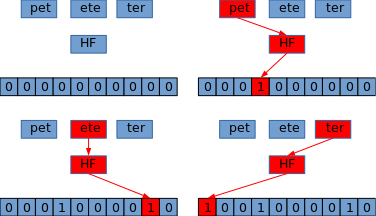
\includegraphics[width=.48\textwidth]{bloom_filter_example_insert.png}
	\caption{Einfügen vom Trigrammen in einen Bloom-Filter}
	\label{fig:add_bf}
	\vspace*{-0.4cm}
\end{wrapfigure}

Um zu überprüfen, ob ein bestimmtes Element im Bloom-Filter enthalten ist, berechnet man seine $k$ Hashwerte.
Ist an einer der $k$ Stellen im Bit-Array eine $0$, so ist dieses Element nicht in der Menge enthalten.
Steht jedoch an allen Positionen eine $1$, so ist der Wert mit einer hohen Wahrscheinlichkeit in der vom Bloom-Filter repräsentierten Menge enthalten.
Aufgrund möglicher Kollisionen kann man im Allgemeinen weder exakt bestimmen,
wie viele disjunkte Elemente ein Bloom-Filter beherbergt, noch sicher sagen, dass ein Element wirklich enthalten ist.

\refnice{Abbildung}{fig:add_bf} visualisiert das Einfügen der Trigramme des Wortes \glqq Peter\grqq.
Es wird veranschaulicht, wie das zuerst leere Bit-Array nach und nach gefüllt wird.
Zur Vereinfachung wird nur eine Hashfunktion verwendet.

\subsubsection{Einsatzszenario in der Entity-Resolution}

Ein Bloom-Filter ist unter den oben beschriebenen Eigenschaften in der Lage, eine Menge zu repräsentieren.
Des weiteren lässt sich ein logisches UND beziehungsweise ein logisches ODER zwischen den Bit-Arrays,
die den Kern einer jeden solchen Datenstrukturen bilden, extrem performant bilden.
Dieser Gedanke führt zu der zentralen Fragestellung dieses Praktikums:\\
Lässt sich die Berechnung der Jaccard-Ähnlichkeit zwischen zwei Mengen durch den Einsatz von Bloom-Filtern
optimieren? Wenn ja, zu welchem Preis?\\

Anschaulich betrachtet bedeutet dies, dass für zwei Mengen $A$ und $B$ - mit entsprechenden Bloom-Filtern $A_{BF}$ bzw.
$B_{BF}$ - der Jaccard-Index gegeben ist durch:

$Jaccard(A_{BF}, B_{BF})$ $=$ $\frac{|A_{BF} \wedge B_{BF}|}{|A_{BF} \vee B_{BF}|}$ $=$
$\frac{\text{geschätzte Anzahl Elemente in } A_{BF} \wedge B_{BF}}{\text{geschätzte Anzahl Elemente in } A_{BF} \vee B_{BF}}$\\
\begin{wrapfigure}{O}{.49\textwidth}
	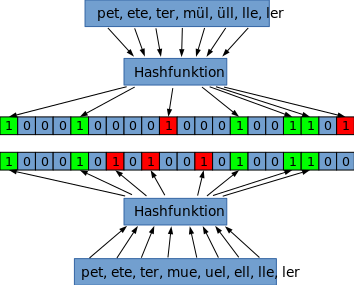
\includegraphics[width=.48\textwidth]{bloom_filter_vergleich.png}
	\caption{Vergleich mit Bloom-Filtern}
	\label{fig:sim_bf}
	\vspace*{-2cm}
\end{wrapfigure}

\refnice{Abbildung}{fig:sim_bf} zeigt diese Funktionsweise für die Berechnung der Ähnlichkeit mittels Bloom-Filtern.
Dabei werden die beiden Instanzen \glqq Peter Müller\grqq~und \glqq Peter Mueller\grqq~vergleichen.
Wenn man beide Bit-Arrays vergleicht, sieht man,
das die Anzahl der UND's gleich 5 und die Anzahl der OR's gleich 10 ist.
Dementsprechend würde die Jaccard-Ähnlichkeit $\frac{5}{10}$ entsprechen.

\newpage
\subsubsection{Gefahren beim Einsatz eines Bloom-Filters}

Für eine approximative Lösung des Entity-Resolution-Problems über den vorgestellten Bloom-Filter-Ansatz
wäre es vorteilhaft, wenn eine allgemeine Beziehung des Jaccard-Indizes für Mengen zu denen mit
Bloom-Filtern existiert.
Insbesondere ein Bezug wie $Jaccard(A, B)$ $\leq$ $Jaccard(A_{BF}, B_{BF})$ wäre wünschenswert.

Leider existieren im Allgemeinen keine derartigen Beziehungen.
Als Ursachen dafür können Kollisionen an verschiedenen Stellen im Workflow identifiziert werden.\\
So bewirken diese beim Aufbau eines Bloom-Filters, dass eine später repräsentierte
Vereinigung kleiner, und der Schnitt größer wird.
Dem entgegen bewirken Kollisionen bei der Bildung der Vereinigung von Bloom-Filtern (logisches oder) eine
unberechtigte Vergrößerung der Mächtigkeit der Vereinigung, während bei dem Schnitt (logisches und)
keine derartigen Effekte auftreten.

\newpage
\section{Vorgehen}
\label{sec:design}

Im Rahmen der Praktikumsaufgabe werden \hyperref[sec:approaches]{verschiedene Vorgehensweisen}
zur Lösung des Entity-Resolution-Problems untersucht.
Um die Vergleichbarkeit der Ansätze zu wahren und eine größere Bandbreite von Auswertungen durchführen zu können,
wollen wir stets Standard-Java-Klassen verwenden.
Dabei sind insbesondere verschiedene Implementierungen der
\href{https://docs.oracle.com/javase/7/docs/api/java/util/List.html}{List-} und
\href{https://docs.oracle.com/javase/7/docs/api/java/util/Set.html}{Set-Schnittstellen} aus dem
\href{http://docs.oracle.com/javase/7/docs/technotes/guides/collections/overview.html}{Collections-Framework}
sowie \href{https://docs.oracle.com/javase/7/docs/api/java/security/MessageDigest.html}{MessageDigest}
und \href{https://docs.oracle.com/javase/7/docs/api/java/util/BitSet.html}{BitSet} relevant.

Zur Lösung der Aufgabe implementieren wir ein Programm (z.Bsp.: PersonEntityResolution.jar), welches für eine Ausführung
die ähnlichen Personen in zwei Personendatensätzen findet.
Dabei soll das Programm durch seine Parametrisierung flexibel aus den oben vorgestellten Lösungsansätzen, inklusive relevanter Details,
wählen können.

Zur vereinfachten Auswertung wird dieses Programm dann durch ein Skript (z.Bsp.: run\_evaluations.sh)
sequentiell für alle interessanten Konstellationen ausgeführt.
Die entstehenden Metadaten sowie Ergebnisse werden aufgehoben.
\refnice{Abbildung}{fig:workflow} stellt dieses Vorgehen schematisch dar.

\begin{figure}[h]
	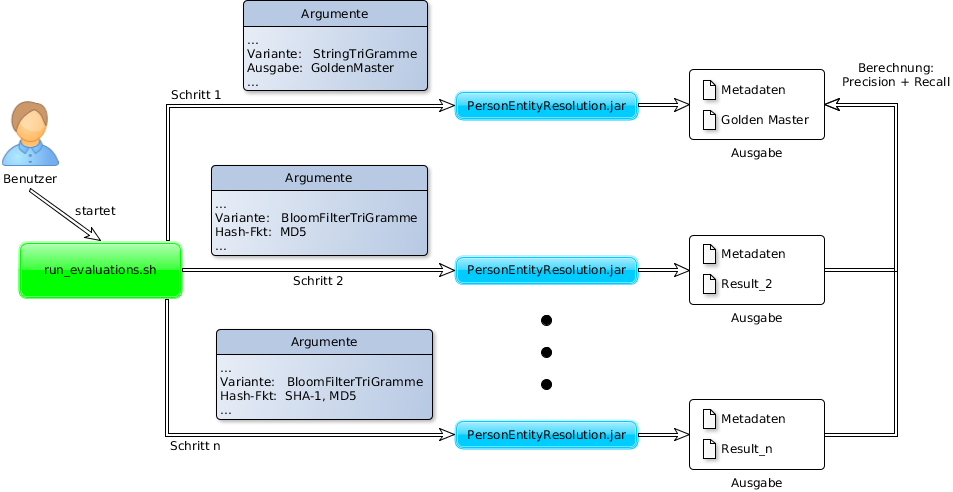
\includegraphics[width=1.01 \textwidth]{evaluation_sketch.png}
	\caption{Workflow zur Evaluierung verschiedener Entity-Resolution-Ansätze}
	\label{fig:workflow}
\end{figure}

So wird im ersten Schritt die Entity-Resolution in der ursprünglichen Variante mit \hyperref[sec:approaches:n-gramm]{String-N-Grammen} durchgeführt.
Die dabei gefundenen Paare von ähnlichen Personen werden für die Ausführungen anderer Konstellationen als Golden-Master abgelegt.

Alle weiteren Ausführungen (2 bis n) stellen nun verschiedene Varianten der Entity-Resolution mit \hyperref[sec:approaches:bloom]{Bloom-Filtern} dar.
Die Menge der anwendbaren Parameter ist vielfältig (\refnice{Abbildung}{fig:parameters} gibt eine Skizze),
was eine ausführliche Auswertung ermöglicht.
Für die Ergebnisse wird dabei stets mittels Precision und Recall gemessen, wie nah sie an die Wahrheit des Golden-Masters heranreichen.

\begin{wrapfigure}{r}{0.49\textwidth}
\begin{tabular}{|l|}
	\hline
	\begin{minipage}{0.46\textwidth}
		\vspace*{0.1cm}
		N-Gramme\\

		\hspace*{-0.4cm}
		\begin{footnotesize}
		\begin{tabular}{l|l}
				Parameter & Wertebereich\\
			\hline
			\hline
				N & TBA\\
			\hline
				Set & $\{$ HashSet, LinkedHashSet $\} \hspace*{0.34cm}$\\
		\end{tabular}
		\end{footnotesize}
	\end{minipage}\\
	\hline
	\hline
	\begin{minipage}{0.46\textwidth}
	\vspace*{0.1cm}
	Bloom-Filter\\

	\hspace*{-0.4cm}
	\begin{footnotesize}
		\begin{tabular}{l|l}
				Parameter & Wertebereich\\
			\hline
			\hline
				N & TBA\\
			\hline
				Attributschachtelung & $\{$ Ja, Nein $\}$\\
			\hline
				Länge Bitliste & \\
			\hline
				Hash-Funktionen & $\{$MD5, SHA, ...$\} \hspace*{0.53cm}$\\
		\end{tabular}
		\end{footnotesize}
	\end{minipage}\\
	\hline
\end{tabular}
\caption{Skizze möglicher Parameter}
\label{fig:parameters}
\end{wrapfigure}

Zusätzlich müssen weitere Kennzahlen erhoben werden.
Dazu gehören im Wesentlichen gemonitorte Details wie Ausführungszeiten und der benötigte Speicherplatz.
Auf Basis der so gesammelten Informationen können ausgiebige Vergleiche der verwendeten Ansätze durchgeführt werden.

Gleichzeitig ist der in \refnice{Abbildung}{fig:workflow} dargestellte Ansatz flexibel genug,
um ohne zusätzlichen Aufwand Tests mehrfach auszuführen und somit Seiteneffekte auszuschließen.

\newpage
\section{Ziele der Implementierung}
\label{sec:implementation}

Die Hauptaufgabe des Praktikums besteht in der Realisierung des in \refnice{Abschnitt}{sec:design}
beschriebenen Programms, sowie der Erstellung der relevanten Auswertungen.
Die bereitzustellenden Aspekte sind dabei in Pflicht- und Optionale Bereiche aufgegliedert,
die im folgenden beschrieben werden.

\subsection{Pflicht: Vergleich verschiedener Strategien}

Das im vorigen Abschnitt beschriebene Vorgehen beruht auf der Idee, dass verschiedene
Implementierungen einer Ähnlichkeitsfunktion zur Entity-Resolution austauschbar
in dem gleichen Workflow ausgeführt werden können.
Um dies zu gewährleisten, wird insbesondere auch der Import der Daten durch die Ähnlichkeitsfunktion so beeinflusst,
dass beim Import die Daten bereits in der von der verwendeten Strategie bevorzugten Datenstruktur bereitgestellt werden.

\refnice{Tabelle}{fig:implementation} beschreibt alle Implementierungen von Ähnlichkeitsfunktionen, die wir im Rahmen der Aufgabe vergleichen wollen.
Viele Ansätze sind redundant vertreten, da wir der Auffassung sind,
dass kleine Implementierungsdetails schwer abzuschätzende Auswirkungen haben können.
Des weiteren existieren verschiedene Implementierungen, die entweder keine oder unvollständige Berechnung ausführen.
Die Motivation dafür besteht in der Möglichkeit, den Workflow hinsichtlich eines isolierten Aspekts zu bewerten.

\begin{figure}[h!]
\begin{tabular}{|l|}
	\hline
	\begin{minipage}{0.999999\textwidth}
		\vspace*{0.1cm}
		\textbf{Komponentenbasierte Personen-Ähnlichkeit}\\

		Ähnlichkeit entspricht arithmetischem Mittel der Jaccard-Ähnlichkeiten der
		N-Gramm-Mengen der Geburtstags-, Name-, Address-Komponenten.\\

		\hspace*{-0.4cm}
		\begin{footnotesize}
		\begin{tabular}{l}
			\hline
				\textbf{\underline{konstante Abbildung auf $0$:}}\\
				\begin{minipage}{0.999999\textwidth} Fokus: Bewertung Import + Transformation \end{minipage}\\
			\hline
				\textbf{\underline{Jaccard-KISS-Ähnlichkeit:}}\\
				Fokus: Lesbarkeit\\
			\hline
				\textbf{\underline{Jaccard-Ähnlichkeit:}}\\
				Fokus: Performance\\
			\hline
				\textbf{\underline{Dritt-Bibliothek-Bloom-Ansatz:}}\\
				Vergleich: Eigenimplementierung vs Verbreitete\\
			\hline
				\textbf{\underline{Bloom-Ansatz (Eigenimplementierung):}}\\
				Mit BitSet\\ 
			\hline
				\textbf{\textbf{Optional: Bloom-Ansatz (Eigenimplementierung):}}\\
				Mit Long-Array\\ 
			\hline
				\textbf{\underline{Optional: Bloom-Ansatz (Eigenimplementierung):}}\\
				Mit Boolean-Array\\ 
		\end{tabular}
		\end{footnotesize}
	\end{minipage}\\
	\hline
	\hline
	\begin{minipage}{0.999999\textwidth}
		\vspace*{0.1cm}
		\textbf{Personen-Ähnlichkeit}\\

		Alle Komponenten einer Person werden in einer gemeinsamen Menge aufbewahrt, wobei die Jaccard-Ähnlichkeiten
		dieser Menge die Ähnlichkeit der Personen entspricht. Ähnlichkeitsfunktionen haben die Bedeutung von oben.\\

		\hspace*{-0.4cm}
		\begin{footnotesize}
		\begin{tabular}{l}
			\hline
				\begin{minipage}{0.999999\textwidth}konstante Abbildung auf $0$\end{minipage}\\
			\hline
				Jaccard-KISS-Ähnlichkeit\\
			\hline
				Jaccard-Ähnlichkeit\\
			\hline
				Dritt-Bibliothek-Bloom-Ansatz\\
			\hline
				Bloom-Ansatz (Eigenimplementierung)\\
			\hline
				Optional: Bloom-Ansatz (Eigenimplementierung)\\
			\hline
				Optional: Bloom-Ansatz (Eigenimplementierung)\\
		\end{tabular}
		\end{footnotesize}
	\end{minipage}\\
	\hline
\end{tabular}
\caption{Übersicht der zu implementierenden Ähnlichkeitsfunktionen}
\label{fig:implementation}
\end{figure}

\subsection{Optional: Parallelisierung}

\begin{itemize}
	\item Ausführen des Workflows in Flink
\end{itemize}


\end{document}


%************************************************************************************************************************
%* begin document
%************************************************************************************************************************
\begin{document}
\thispagestyle{empty}

\begin{center}
\large

\vspace{1cm}
\textbf{\sffamily	Universität Leipzig\\
			Fakultät für Mathematik und Informatik\\
			Institut für Informatik\\}

\vspace{2cm}
{\Large\textbf{\sffamily Speed up Entity Resolution with Bit Arrays}}


\large

Big Data Praktikum
\vspace{1cm}
\end{center}

\textbf{Einleitung}:\\
Das Ziel des Praktikums besteht darin, durch experimentelle Auswertungen zwei Ansätze zur Entity-Resolution miteinander
zu vergleichen.
Der erste Vertreter ist dabei die Jaccard-Ähnlichkeit von N-Grammen.
Dieses Vorgehen liefert gute Ergebnisse, lässt jedoch aus Sicht der Ausführungszeit insbesondere für große Datenmengen Wünsche offen.

Aus diesem Grund wird die zweite Strategie auf der Basis von Bloom-Filtern realisiert.
Bloom-Filter sind dabei Datenstrukturen, die approximativ und sehr effizient entscheiden können,
ob ein gegebenes Element in einer Menge enthalten ist.
Durch diese Objekte sollen damit die für die Jaccard-Ähnlichkeit notwendigen Berechnungen effizient approximiert werden.

Die Hoffnung besteht dabei darin, dass dieser Ansatz möglichst wenig Genauigkeit einbüßt,
und dabei signifikante Verbesserungen in Bezug auf die Ausführungszeit liefert.


\vfill

{\large
\begin{tabular}{p{7cm} ll}
&\\
\small
Leipzig, Mai 2017 & \small vorgelegt von\\
				& \small Maik Fröbe & \small 2515360\\

				& \small Moritz Engelmann & \small 2527532\\
\end{tabular}}

\begin{tabular}{p{7cm} l}
&\\
\small
Betreuer:	& \small Ziad Sehili \\
			& \small Fakultät für Mathematik und Informatik\\
			& \small Abteilung Datenbanken
\end{tabular} 

\newpage

\pagenumbering{arabic}

%************************************************************************************************************************
%* main sections
%************************************************************************************************************************
\newpage
\section{Entity-Resolution}
\label{sec:approaches}

Zwei eigentlich identische Objekte können sich durch verschiedene Schreibweisen,
Abkürzungen, oder der Verwendung unterschiedlicher Persistierungen unterscheiden.
So können z.B. die beiden Instanzen \glqq Peter Müller\grqq und \glqq Peter Mueller\grqq die selbe Person darstellen,
obwohl sie unterschiedlich geschrieben sind.

Ziel der Entity-Resolution ist es durch automatische Verfahren herauszufinden,
ob zwei Instanzen aus verschiedenen Datensätzen dasselbe Objekt in der realen Welt repräsentieren.
Das ist z.B. nötig, wenn man verschiedene Datenquellen zusammenführen oder eine Datenbereinigung vornehmen möchte.
Dazu ist es nötig, geeignete Methoden zu verwenden bzw. zu entwickeln,
welche identische Instanzen möglichst schnell und genau identifizieren können.
Im folgenden sollen zwei Verfahren vorgestellt und in der weiteren Arbeit verglichen werden.

\subsection{Entity-Resolution mit N-Grammen}
\label{sec:approaches:n-gramm}

Für die Berechnung von Ähnlichkeiten mittels N-Grammen müssen aus den zu vergleichenden Instanzen zuerst N-Gramme erzeugt werden.
Beispielsweise werden aus den beiden Instanzen \glqq Peter Müller\grqq und \glqq Peter Mueller\grqq die folgenden Trigramme erzeugt:
\input{n-gramms.conf}

Mittels der Jaccard-Ähnlichkeit kann nun die Ähnlichkeit von A und B berechnet werden:

$Jaccard(A, B)$ $=$ $\frac{A \cap B}{A \cup B}$ $=$ $\frac{5}{10}$ $=$ $\frac{1}{2}$

Wenn man nun einen Schwellwert festlegt und die berechnete Ähnlichkeit ist größer oder gleich diesem Schwellwert,
so geht man davon aus, das es sich um die selben Instanzen handelt.

\subsection{Entity-Resolution mit N-Grammen unter Verwendung von Bloom-Filtern}
\label{sec:approaches:bloom}

Eine zentrale Rolle bezüglich der Performance der Entity-Resolution stellt der Aufwand für die Bestimmung der Ähnlichkeit zweier Objekte dar.
Insbesondere ein wie oben vorgestellter Ansatz, der auf der Berechnung des Jaccard-Index zwischen Mengen basiert,
ist aufgrund teurer Schnitt- und Vereinigungs-Berechnungen aufwändig.
Ein alternativer Ansatz stellt eine approximative Lösung, zum Beispiel unter Verwendung von Bloom-Filtern, dar.

\subsubsection{Bloom-Filter}

Ein Bloom-Filter ist eine Datenstruktur, die effizient - aber dafür approximativ - entscheidet,
ob ein beliebiges Element in einer, durch den Bloom-Filter repräsentierten, Menge enthalten ist.
Für einen Bloom-Filter $A_{BF}$ einer Menge $A$ gilt dabei stets: $x \in A$ $\Rightarrow$ $x \in A_{BF}$.

Realisiert wird ein solches Objekt mit einem Bit-Array der Länge $n$,
sowie einer Anzahl $k$ unterschiedlicher Hashfunktionen.
Diese Hashfunktionen haben jeweils einen Wertebereich von $0$ bis $n - 1$.
Initial ist der Bit-Array mit Nullen gefüllt.

Anschließen werden die Elemente der verwalteten Menge eingefügt.
Dazu werden mittels der $k$ verschiedenen Hashfunktionen $k$ Hashwerte ermittelt.
Jeder dieser Hashwerte wird nun auf die entsprechende Position im Bit-Array übertragen.
Dazu werden diese Positionen auf $1$ gesetzt.
Wenn eine Position schon durch einen anderen Hashwert auf $1$ gesetzt worden ist,
kommt es zu einer Kollision und diese Position wird auf $1$ belassen.

\begin{wrapfigure}{O}{.49\textwidth}
	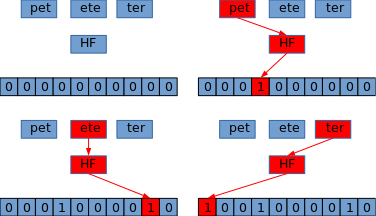
\includegraphics[width=.48\textwidth]{bloom_filter_example_insert.png}
	\caption{Einfügen vom Trigrammen in einen Bloom-Filter}
	\label{fig:add_bf}
	\vspace*{-0.4cm}
\end{wrapfigure}

Um zu überprüfen, ob ein bestimmtes Element im Bloom-Filter enthalten ist, berechnet man seine $k$ Hashwerte.
Ist an einer der $k$ Stellen im Bit-Array eine $0$, so ist dieses Element nicht in der Menge enthalten.
Steht jedoch an allen Positionen eine $1$, so ist der Wert mit einer hohen Wahrscheinlichkeit in der vom Bloom-Filter repräsentierten Menge enthalten.
Aufgrund möglicher Kollisionen kann man im Allgemeinen weder exakt bestimmen,
wie viele disjunkte Elemente ein Bloom-Filter beherbergt, noch sicher sagen, dass ein Element wirklich enthalten ist.

\refnice{Abbildung}{fig:add_bf} visualisiert das Einfügen der Trigramme des Wortes \glqq Peter\grqq.
Es wird veranschaulicht, wie das zuerst leere Bit-Array nach und nach gefüllt wird.
Zur Vereinfachung wird nur eine Hashfunktion verwendet.

\subsubsection{Einsatzszenario in der Entity-Resolution}

Ein Bloom-Filter ist unter den oben beschriebenen Eigenschaften in der Lage, eine Menge zu repräsentieren.
Des weiteren lässt sich ein logisches UND beziehungsweise ein logisches ODER zwischen den Bit-Arrays,
die den Kern einer jeden solchen Datenstrukturen bilden, extrem performant bilden.
Dieser Gedanke führt zu der zentralen Fragestellung dieses Praktikums:\\
Lässt sich die Berechnung der Jaccard-Ähnlichkeit zwischen zwei Mengen durch den Einsatz von Bloom-Filtern
optimieren? Wenn ja, zu welchem Preis?\\

Anschaulich betrachtet bedeutet dies, dass für zwei Mengen $A$ und $B$ - mit entsprechenden Bloom-Filtern $A_{BF}$ bzw.
$B_{BF}$ - der Jaccard-Index gegeben ist durch:

$Jaccard(A_{BF}, B_{BF})$ $=$ $\frac{|A_{BF} \wedge B_{BF}|}{|A_{BF} \vee B_{BF}|}$ $=$
$\frac{\text{geschätzte Anzahl Elemente in } A_{BF} \wedge B_{BF}}{\text{geschätzte Anzahl Elemente in } A_{BF} \vee B_{BF}}$\\
\begin{wrapfigure}{O}{.49\textwidth}
	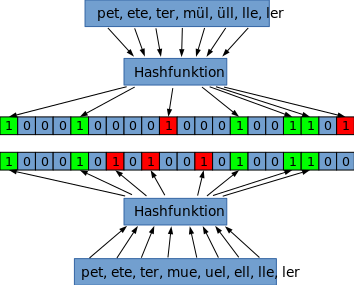
\includegraphics[width=.48\textwidth]{bloom_filter_vergleich.png}
	\caption{Vergleich mit Bloom-Filtern}
	\label{fig:sim_bf}
	\vspace*{-2cm}
\end{wrapfigure}

\refnice{Abbildung}{fig:sim_bf} zeigt diese Funktionsweise für die Berechnung der Ähnlichkeit mittels Bloom-Filtern.
Dabei werden die beiden Instanzen \glqq Peter Müller\grqq~und \glqq Peter Mueller\grqq~vergleichen.
Wenn man beide Bit-Arrays vergleicht, sieht man,
das die Anzahl der UND's gleich 5 und die Anzahl der OR's gleich 10 ist.
Dementsprechend würde die Jaccard-Ähnlichkeit $\frac{5}{10}$ entsprechen.

\newpage
\subsubsection{Gefahren beim Einsatz eines Bloom-Filters}

Für eine approximative Lösung des Entity-Resolution-Problems über den vorgestellten Bloom-Filter-Ansatz
wäre es vorteilhaft, wenn eine allgemeine Beziehung des Jaccard-Indizes für Mengen zu denen mit
Bloom-Filtern existiert.
Insbesondere ein Bezug wie $Jaccard(A, B)$ $\leq$ $Jaccard(A_{BF}, B_{BF})$ wäre wünschenswert.

Leider existieren im Allgemeinen keine derartigen Beziehungen.
Als Ursachen dafür können Kollisionen an verschiedenen Stellen im Workflow identifiziert werden.\\
So bewirken diese beim Aufbau eines Bloom-Filters, dass eine später repräsentierte
Vereinigung kleiner, und der Schnitt größer wird.
Dem entgegen bewirken Kollisionen bei der Bildung der Vereinigung von Bloom-Filtern (logisches oder) eine
unberechtigte Vergrößerung der Mächtigkeit der Vereinigung, während bei dem Schnitt (logisches und)
keine derartigen Effekte auftreten.

\newpage
\section{Vorgehen}
\label{sec:design}

Im Rahmen der Praktikumsaufgabe werden \hyperref[sec:approaches]{verschiedene Vorgehensweisen}
zur Lösung des Entity-Resolution-Problems untersucht.
Um die Vergleichbarkeit der Ansätze zu wahren und eine größere Bandbreite von Auswertungen durchführen zu können,
wollen wir stets Standard-Java-Klassen verwenden.
Dabei sind insbesondere verschiedene Implementierungen der
\href{https://docs.oracle.com/javase/7/docs/api/java/util/List.html}{List-} und
\href{https://docs.oracle.com/javase/7/docs/api/java/util/Set.html}{Set-Schnittstellen} aus dem
\href{http://docs.oracle.com/javase/7/docs/technotes/guides/collections/overview.html}{Collections-Framework}
sowie \href{https://docs.oracle.com/javase/7/docs/api/java/security/MessageDigest.html}{MessageDigest}
und \href{https://docs.oracle.com/javase/7/docs/api/java/util/BitSet.html}{BitSet} relevant.

Zur Lösung der Aufgabe implementieren wir ein Programm (z.Bsp.: PersonEntityResolution.jar), welches für eine Ausführung
die ähnlichen Personen in zwei Personendatensätzen findet.
Dabei soll das Programm durch seine Parametrisierung flexibel aus den oben vorgestellten Lösungsansätzen, inklusive relevanter Details,
wählen können.

Zur vereinfachten Auswertung wird dieses Programm dann durch ein Skript (z.Bsp.: run\_evaluations.sh)
sequentiell für alle interessanten Konstellationen ausgeführt.
Die entstehenden Metadaten sowie Ergebnisse werden aufgehoben.
\refnice{Abbildung}{fig:workflow} stellt dieses Vorgehen schematisch dar.

\begin{figure}[h]
	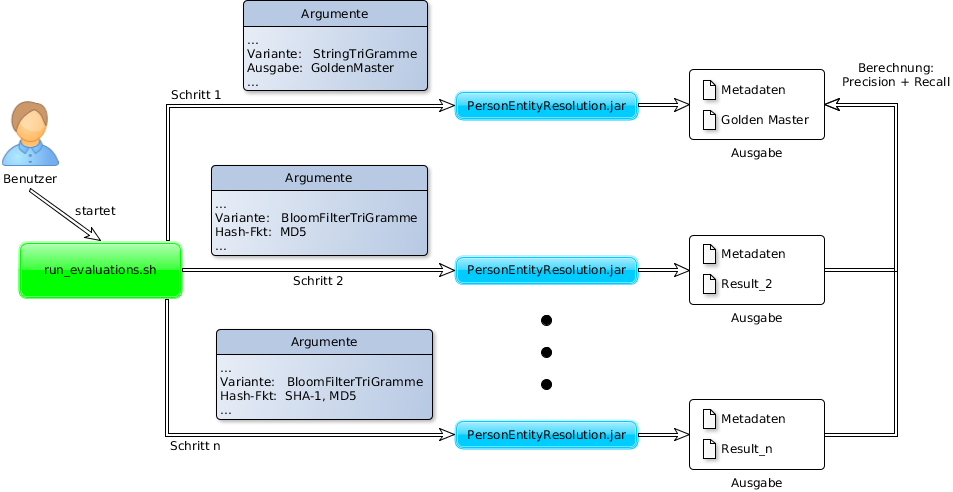
\includegraphics[width=1.01 \textwidth]{evaluation_sketch.png}
	\caption{Workflow zur Evaluierung verschiedener Entity-Resolution-Ansätze}
	\label{fig:workflow}
\end{figure}

So wird im ersten Schritt die Entity-Resolution in der ursprünglichen Variante mit \hyperref[sec:approaches:n-gramm]{String-N-Grammen} durchgeführt.
Die dabei gefundenen Paare von ähnlichen Personen werden für die Ausführungen anderer Konstellationen als Golden-Master abgelegt.

Alle weiteren Ausführungen (2 bis n) stellen nun verschiedene Varianten der Entity-Resolution mit \hyperref[sec:approaches:bloom]{Bloom-Filtern} dar.
Die Menge der anwendbaren Parameter ist vielfältig (\refnice{Abbildung}{fig:parameters} gibt eine Skizze),
was eine ausführliche Auswertung ermöglicht.
Für die Ergebnisse wird dabei stets mittels Precision und Recall gemessen, wie nah sie an die Wahrheit des Golden-Masters heranreichen.

\begin{wrapfigure}{r}{0.49\textwidth}
\begin{tabular}{|l|}
	\hline
	\begin{minipage}{0.46\textwidth}
		\vspace*{0.1cm}
		N-Gramme\\

		\hspace*{-0.4cm}
		\begin{footnotesize}
		\begin{tabular}{l|l}
				Parameter & Wertebereich\\
			\hline
			\hline
				N & TBA\\
			\hline
				Set & $\{$ HashSet, LinkedHashSet $\} \hspace*{0.34cm}$\\
		\end{tabular}
		\end{footnotesize}
	\end{minipage}\\
	\hline
	\hline
	\begin{minipage}{0.46\textwidth}
	\vspace*{0.1cm}
	Bloom-Filter\\

	\hspace*{-0.4cm}
	\begin{footnotesize}
		\begin{tabular}{l|l}
				Parameter & Wertebereich\\
			\hline
			\hline
				N & TBA\\
			\hline
				Attributschachtelung & $\{$ Ja, Nein $\}$\\
			\hline
				Länge Bitliste & \\
			\hline
				Hash-Funktionen & $\{$MD5, SHA, ...$\} \hspace*{0.53cm}$\\
		\end{tabular}
		\end{footnotesize}
	\end{minipage}\\
	\hline
\end{tabular}
\caption{Skizze möglicher Parameter}
\label{fig:parameters}
\end{wrapfigure}

Zusätzlich müssen weitere Kennzahlen erhoben werden.
Dazu gehören im Wesentlichen gemonitorte Details wie Ausführungszeiten und der benötigte Speicherplatz.
Auf Basis der so gesammelten Informationen können ausgiebige Vergleiche der verwendeten Ansätze durchgeführt werden.

Gleichzeitig ist der in \refnice{Abbildung}{fig:workflow} dargestellte Ansatz flexibel genug,
um ohne zusätzlichen Aufwand Tests mehrfach auszuführen und somit Seiteneffekte auszuschließen.

\newpage
\section{Ziele der Implementierung}
\label{sec:implementation}

Die Hauptaufgabe des Praktikums besteht in der Realisierung des in \refnice{Abschnitt}{sec:design}
beschriebenen Programms, sowie der Erstellung der relevanten Auswertungen.
Die bereitzustellenden Aspekte sind dabei in Pflicht- und Optionale Bereiche aufgegliedert,
die im folgenden beschrieben werden.

\subsection{Pflicht: Vergleich verschiedener Strategien}

Das im vorigen Abschnitt beschriebene Vorgehen beruht auf der Idee, dass verschiedene
Implementierungen einer Ähnlichkeitsfunktion zur Entity-Resolution austauschbar
in dem gleichen Workflow ausgeführt werden können.
Um dies zu gewährleisten, wird insbesondere auch der Import der Daten durch die Ähnlichkeitsfunktion so beeinflusst,
dass beim Import die Daten bereits in der von der verwendeten Strategie bevorzugten Datenstruktur bereitgestellt werden.

\refnice{Tabelle}{fig:implementation} beschreibt alle Implementierungen von Ähnlichkeitsfunktionen, die wir im Rahmen der Aufgabe vergleichen wollen.
Viele Ansätze sind redundant vertreten, da wir der Auffassung sind,
dass kleine Implementierungsdetails schwer abzuschätzende Auswirkungen haben können.
Des weiteren existieren verschiedene Implementierungen, die entweder keine oder unvollständige Berechnung ausführen.
Die Motivation dafür besteht in der Möglichkeit, den Workflow hinsichtlich eines isolierten Aspekts zu bewerten.

\begin{figure}[h!]
\begin{tabular}{|l|}
	\hline
	\begin{minipage}{0.999999\textwidth}
		\vspace*{0.1cm}
		\textbf{Komponentenbasierte Personen-Ähnlichkeit}\\

		Ähnlichkeit entspricht arithmetischem Mittel der Jaccard-Ähnlichkeiten der
		N-Gramm-Mengen der Geburtstags-, Name-, Address-Komponenten.\\

		\hspace*{-0.4cm}
		\begin{footnotesize}
		\begin{tabular}{l}
			\hline
				\textbf{\underline{konstante Abbildung auf $0$:}}\\
				\begin{minipage}{0.999999\textwidth} Fokus: Bewertung Import + Transformation \end{minipage}\\
			\hline
				\textbf{\underline{Jaccard-KISS-Ähnlichkeit:}}\\
				Fokus: Lesbarkeit\\
			\hline
				\textbf{\underline{Jaccard-Ähnlichkeit:}}\\
				Fokus: Performance\\
			\hline
				\textbf{\underline{Dritt-Bibliothek-Bloom-Ansatz:}}\\
				Vergleich: Eigenimplementierung vs Verbreitete\\
			\hline
				\textbf{\underline{Bloom-Ansatz (Eigenimplementierung):}}\\
				Mit BitSet\\ 
			\hline
				\textbf{\textbf{Optional: Bloom-Ansatz (Eigenimplementierung):}}\\
				Mit Long-Array\\ 
			\hline
				\textbf{\underline{Optional: Bloom-Ansatz (Eigenimplementierung):}}\\
				Mit Boolean-Array\\ 
		\end{tabular}
		\end{footnotesize}
	\end{minipage}\\
	\hline
	\hline
	\begin{minipage}{0.999999\textwidth}
		\vspace*{0.1cm}
		\textbf{Personen-Ähnlichkeit}\\

		Alle Komponenten einer Person werden in einer gemeinsamen Menge aufbewahrt, wobei die Jaccard-Ähnlichkeiten
		dieser Menge die Ähnlichkeit der Personen entspricht. Ähnlichkeitsfunktionen haben die Bedeutung von oben.\\

		\hspace*{-0.4cm}
		\begin{footnotesize}
		\begin{tabular}{l}
			\hline
				\begin{minipage}{0.999999\textwidth}konstante Abbildung auf $0$\end{minipage}\\
			\hline
				Jaccard-KISS-Ähnlichkeit\\
			\hline
				Jaccard-Ähnlichkeit\\
			\hline
				Dritt-Bibliothek-Bloom-Ansatz\\
			\hline
				Bloom-Ansatz (Eigenimplementierung)\\
			\hline
				Optional: Bloom-Ansatz (Eigenimplementierung)\\
			\hline
				Optional: Bloom-Ansatz (Eigenimplementierung)\\
		\end{tabular}
		\end{footnotesize}
	\end{minipage}\\
	\hline
\end{tabular}
\caption{Übersicht der zu implementierenden Ähnlichkeitsfunktionen}
\label{fig:implementation}
\end{figure}

\subsection{Optional: Parallelisierung}

\begin{itemize}
	\item Ausführen des Workflows in Flink
\end{itemize}


\end{document}


%************************************************************************************************************************
%* begin document
%************************************************************************************************************************
\begin{document}
\thispagestyle{empty}

\begin{center}
\large

\vspace{1cm}
\textbf{\sffamily	Universität Leipzig\\
			Fakultät für Mathematik und Informatik\\
			Institut für Informatik\\}

\vspace{2cm}
{\Large\textbf{\sffamily Speed up Entity Resolution with Bit Arrays}}


\large

Big Data Praktikum
\vspace{1cm}
\end{center}

\textbf{Einleitung}:\\
Das Ziel des Praktikums besteht darin, durch experimentelle Auswertungen zwei Ansätze zur Entity-Resolution miteinander
zu vergleichen.
Der erste Vertreter ist dabei die Jaccard-Ähnlichkeit von N-Grammen.
Dieses Vorgehen liefert gute Ergebnisse, lässt jedoch aus Sicht der Ausführungszeit insbesondere für große Datenmengen Wünsche offen.

Aus diesem Grund wird die zweite Strategie auf der Basis von Bloom-Filtern realisiert.
Bloom-Filter sind dabei Datenstrukturen, die approximativ und sehr effizient entscheiden können,
ob ein gegebenes Element in einer Menge enthalten ist.
Durch diese Objekte sollen damit die für die Jaccard-Ähnlichkeit notwendigen Berechnungen effizient approximiert werden.

Die Hoffnung besteht dabei darin, dass dieser Ansatz möglichst wenig Genauigkeit einbüßt,
und dabei signifikante Verbesserungen in Bezug auf die Ausführungszeit liefert.


\vfill

{\large
\begin{tabular}{p{7cm} ll}
&\\
\small
Leipzig, Mai 2017 & \small vorgelegt von\\
				& \small Maik Fröbe & \small 2515360\\

				& \small Moritz Engelmann & \small 2527532\\
\end{tabular}}

\begin{tabular}{p{7cm} l}
&\\
\small
Betreuer:	& \small Ziad Sehili \\
			& \small Fakultät für Mathematik und Informatik\\
			& \small Abteilung Datenbanken
\end{tabular} 

\newpage

\pagenumbering{arabic}

%************************************************************************************************************************
%* main sections
%************************************************************************************************************************
\newpage
\section{Entity-Resolution}
\label{sec:approaches}

Zwei eigentlich identische Objekte können sich durch verschiedene Schreibweisen,
Abkürzungen, oder der Verwendung unterschiedlicher Persistierungen unterscheiden.
So können z.B. die beiden Instanzen \glqq Peter Müller\grqq und \glqq Peter Mueller\grqq die selbe Person darstellen,
obwohl sie unterschiedlich geschrieben sind.

Ziel der Entity-Resolution ist es durch automatische Verfahren herauszufinden,
ob zwei Instanzen aus verschiedenen Datensätzen dasselbe Objekt in der realen Welt repräsentieren.
Das ist z.B. nötig, wenn man verschiedene Datenquellen zusammenführen oder eine Datenbereinigung vornehmen möchte.
Dazu ist es nötig, geeignete Methoden zu verwenden bzw. zu entwickeln,
welche identische Instanzen möglichst schnell und genau identifizieren können.
Im folgenden sollen zwei Verfahren vorgestellt und in der weiteren Arbeit verglichen werden.

\subsection{Entity-Resolution mit N-Grammen}
\label{sec:approaches:n-gramm}

Für die Berechnung von Ähnlichkeiten mittels N-Grammen müssen aus den zu vergleichenden Instanzen zuerst N-Gramme erzeugt werden.
Beispielsweise werden aus den beiden Instanzen \glqq Peter Müller\grqq und \glqq Peter Mueller\grqq die folgenden Trigramme erzeugt:
\input{n-gramms.conf}

Mittels der Jaccard-Ähnlichkeit kann nun die Ähnlichkeit von A und B berechnet werden:

$Jaccard(A, B)$ $=$ $\frac{A \cap B}{A \cup B}$ $=$ $\frac{5}{10}$ $=$ $\frac{1}{2}$

Wenn man nun einen Schwellwert festlegt und die berechnete Ähnlichkeit ist größer oder gleich diesem Schwellwert,
so geht man davon aus, das es sich um die selben Instanzen handelt.

\subsection{Entity-Resolution mit N-Grammen unter Verwendung von Bloom-Filtern}
\label{sec:approaches:bloom}

Eine zentrale Rolle bezüglich der Performance der Entity-Resolution stellt der Aufwand für die Bestimmung der Ähnlichkeit zweier Objekte dar.
Insbesondere ein wie oben vorgestellter Ansatz, der auf der Berechnung des Jaccard-Index zwischen Mengen basiert,
ist aufgrund teurer Schnitt- und Vereinigungs-Berechnungen aufwändig.
Ein alternativer Ansatz stellt eine approximative Lösung, zum Beispiel unter Verwendung von Bloom-Filtern, dar.

\subsubsection{Bloom-Filter}

Ein Bloom-Filter ist eine Datenstruktur, die effizient - aber dafür approximativ - entscheidet,
ob ein beliebiges Element in einer, durch den Bloom-Filter repräsentierten, Menge enthalten ist.
Für einen Bloom-Filter $A_{BF}$ einer Menge $A$ gilt dabei stets: $x \in A$ $\Rightarrow$ $x \in A_{BF}$.

Realisiert wird ein solches Objekt mit einem Bit-Array der Länge $n$,
sowie einer Anzahl $k$ unterschiedlicher Hashfunktionen.
Diese Hashfunktionen haben jeweils einen Wertebereich von $0$ bis $n - 1$.
Initial ist der Bit-Array mit Nullen gefüllt.

Anschließen werden die Elemente der verwalteten Menge eingefügt.
Dazu werden mittels der $k$ verschiedenen Hashfunktionen $k$ Hashwerte ermittelt.
Jeder dieser Hashwerte wird nun auf die entsprechende Position im Bit-Array übertragen.
Dazu werden diese Positionen auf $1$ gesetzt.
Wenn eine Position schon durch einen anderen Hashwert auf $1$ gesetzt worden ist,
kommt es zu einer Kollision und diese Position wird auf $1$ belassen.

\begin{wrapfigure}{O}{.49\textwidth}
	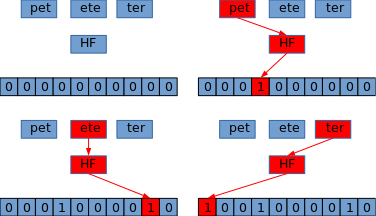
\includegraphics[width=.48\textwidth]{bloom_filter_example_insert.png}
	\caption{Einfügen vom Trigrammen in einen Bloom-Filter}
	\label{fig:add_bf}
	\vspace*{-0.4cm}
\end{wrapfigure}

Um zu überprüfen, ob ein bestimmtes Element im Bloom-Filter enthalten ist, berechnet man seine $k$ Hashwerte.
Ist an einer der $k$ Stellen im Bit-Array eine $0$, so ist dieses Element nicht in der Menge enthalten.
Steht jedoch an allen Positionen eine $1$, so ist der Wert mit einer hohen Wahrscheinlichkeit in der vom Bloom-Filter repräsentierten Menge enthalten.
Aufgrund möglicher Kollisionen kann man im Allgemeinen weder exakt bestimmen,
wie viele disjunkte Elemente ein Bloom-Filter beherbergt, noch sicher sagen, dass ein Element wirklich enthalten ist.

\refnice{Abbildung}{fig:add_bf} visualisiert das Einfügen der Trigramme des Wortes \glqq Peter\grqq.
Es wird veranschaulicht, wie das zuerst leere Bit-Array nach und nach gefüllt wird.
Zur Vereinfachung wird nur eine Hashfunktion verwendet.

\subsubsection{Einsatzszenario in der Entity-Resolution}

Ein Bloom-Filter ist unter den oben beschriebenen Eigenschaften in der Lage, eine Menge zu repräsentieren.
Des weiteren lässt sich ein logisches UND beziehungsweise ein logisches ODER zwischen den Bit-Arrays,
die den Kern einer jeden solchen Datenstrukturen bilden, extrem performant bilden.
Dieser Gedanke führt zu der zentralen Fragestellung dieses Praktikums:\\
Lässt sich die Berechnung der Jaccard-Ähnlichkeit zwischen zwei Mengen durch den Einsatz von Bloom-Filtern
optimieren? Wenn ja, zu welchem Preis?\\

Anschaulich betrachtet bedeutet dies, dass für zwei Mengen $A$ und $B$ - mit entsprechenden Bloom-Filtern $A_{BF}$ bzw.
$B_{BF}$ - der Jaccard-Index gegeben ist durch:

$Jaccard(A_{BF}, B_{BF})$ $=$ $\frac{|A_{BF} \wedge B_{BF}|}{|A_{BF} \vee B_{BF}|}$ $=$
$\frac{\text{geschätzte Anzahl Elemente in } A_{BF} \wedge B_{BF}}{\text{geschätzte Anzahl Elemente in } A_{BF} \vee B_{BF}}$\\
\begin{wrapfigure}{O}{.49\textwidth}
	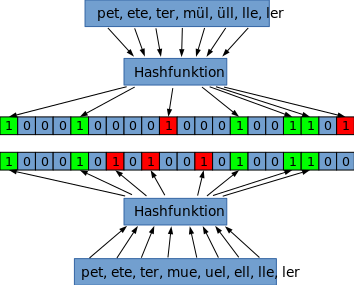
\includegraphics[width=.48\textwidth]{bloom_filter_vergleich.png}
	\caption{Vergleich mit Bloom-Filtern}
	\label{fig:sim_bf}
	\vspace*{-2cm}
\end{wrapfigure}

\refnice{Abbildung}{fig:sim_bf} zeigt diese Funktionsweise für die Berechnung der Ähnlichkeit mittels Bloom-Filtern.
Dabei werden die beiden Instanzen \glqq Peter Müller\grqq~und \glqq Peter Mueller\grqq~vergleichen.
Wenn man beide Bit-Arrays vergleicht, sieht man,
das die Anzahl der UND's gleich 5 und die Anzahl der OR's gleich 10 ist.
Dementsprechend würde die Jaccard-Ähnlichkeit $\frac{5}{10}$ entsprechen.

\newpage
\subsubsection{Gefahren beim Einsatz eines Bloom-Filters}

Für eine approximative Lösung des Entity-Resolution-Problems über den vorgestellten Bloom-Filter-Ansatz
wäre es vorteilhaft, wenn eine allgemeine Beziehung des Jaccard-Indizes für Mengen zu denen mit
Bloom-Filtern existiert.
Insbesondere ein Bezug wie $Jaccard(A, B)$ $\leq$ $Jaccard(A_{BF}, B_{BF})$ wäre wünschenswert.

Leider existieren im Allgemeinen keine derartigen Beziehungen.
Als Ursachen dafür können Kollisionen an verschiedenen Stellen im Workflow identifiziert werden.\\
So bewirken diese beim Aufbau eines Bloom-Filters, dass eine später repräsentierte
Vereinigung kleiner, und der Schnitt größer wird.
Dem entgegen bewirken Kollisionen bei der Bildung der Vereinigung von Bloom-Filtern (logisches oder) eine
unberechtigte Vergrößerung der Mächtigkeit der Vereinigung, während bei dem Schnitt (logisches und)
keine derartigen Effekte auftreten.

\newpage
\section{Vorgehen}
\label{sec:design}

Im Rahmen der Praktikumsaufgabe werden \hyperref[sec:approaches]{verschiedene Vorgehensweisen}
zur Lösung des Entity-Resolution-Problems untersucht.
Um die Vergleichbarkeit der Ansätze zu wahren und eine größere Bandbreite von Auswertungen durchführen zu können,
wollen wir stets Standard-Java-Klassen verwenden.
Dabei sind insbesondere verschiedene Implementierungen der
\href{https://docs.oracle.com/javase/7/docs/api/java/util/List.html}{List-} und
\href{https://docs.oracle.com/javase/7/docs/api/java/util/Set.html}{Set-Schnittstellen} aus dem
\href{http://docs.oracle.com/javase/7/docs/technotes/guides/collections/overview.html}{Collections-Framework}
sowie \href{https://docs.oracle.com/javase/7/docs/api/java/security/MessageDigest.html}{MessageDigest}
und \href{https://docs.oracle.com/javase/7/docs/api/java/util/BitSet.html}{BitSet} relevant.

Zur Lösung der Aufgabe implementieren wir ein Programm (z.Bsp.: PersonEntityResolution.jar), welches für eine Ausführung
die ähnlichen Personen in zwei Personendatensätzen findet.
Dabei soll das Programm durch seine Parametrisierung flexibel aus den oben vorgestellten Lösungsansätzen, inklusive relevanter Details,
wählen können.

Zur vereinfachten Auswertung wird dieses Programm dann durch ein Skript (z.Bsp.: run\_evaluations.sh)
sequentiell für alle interessanten Konstellationen ausgeführt.
Die entstehenden Metadaten sowie Ergebnisse werden aufgehoben.
\refnice{Abbildung}{fig:workflow} stellt dieses Vorgehen schematisch dar.

\begin{figure}[h]
	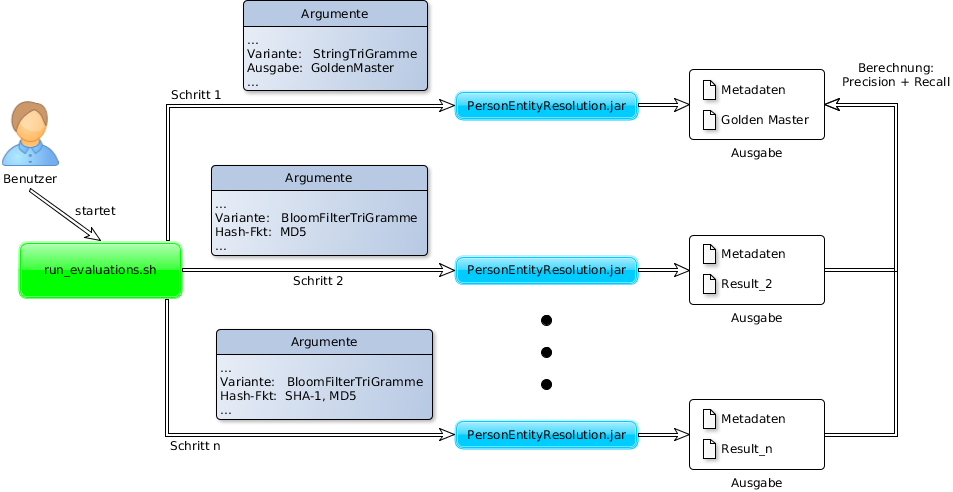
\includegraphics[width=1.01 \textwidth]{evaluation_sketch.png}
	\caption{Workflow zur Evaluierung verschiedener Entity-Resolution-Ansätze}
	\label{fig:workflow}
\end{figure}

So wird im ersten Schritt die Entity-Resolution in der ursprünglichen Variante mit \hyperref[sec:approaches:n-gramm]{String-N-Grammen} durchgeführt.
Die dabei gefundenen Paare von ähnlichen Personen werden für die Ausführungen anderer Konstellationen als Golden-Master abgelegt.

Alle weiteren Ausführungen (2 bis n) stellen nun verschiedene Varianten der Entity-Resolution mit \hyperref[sec:approaches:bloom]{Bloom-Filtern} dar.
Die Menge der anwendbaren Parameter ist vielfältig (\refnice{Abbildung}{fig:parameters} gibt eine Skizze),
was eine ausführliche Auswertung ermöglicht.
Für die Ergebnisse wird dabei stets mittels Precision und Recall gemessen, wie nah sie an die Wahrheit des Golden-Masters heranreichen.

\begin{wrapfigure}{r}{0.49\textwidth}
\begin{tabular}{|l|}
	\hline
	\begin{minipage}{0.46\textwidth}
		\vspace*{0.1cm}
		N-Gramme\\

		\hspace*{-0.4cm}
		\begin{footnotesize}
		\begin{tabular}{l|l}
				Parameter & Wertebereich\\
			\hline
			\hline
				N & TBA\\
			\hline
				Set & $\{$ HashSet, LinkedHashSet $\} \hspace*{0.34cm}$\\
		\end{tabular}
		\end{footnotesize}
	\end{minipage}\\
	\hline
	\hline
	\begin{minipage}{0.46\textwidth}
	\vspace*{0.1cm}
	Bloom-Filter\\

	\hspace*{-0.4cm}
	\begin{footnotesize}
		\begin{tabular}{l|l}
				Parameter & Wertebereich\\
			\hline
			\hline
				N & TBA\\
			\hline
				Attributschachtelung & $\{$ Ja, Nein $\}$\\
			\hline
				Länge Bitliste & \\
			\hline
				Hash-Funktionen & $\{$MD5, SHA, ...$\} \hspace*{0.53cm}$\\
		\end{tabular}
		\end{footnotesize}
	\end{minipage}\\
	\hline
\end{tabular}
\caption{Skizze möglicher Parameter}
\label{fig:parameters}
\end{wrapfigure}

Zusätzlich müssen weitere Kennzahlen erhoben werden.
Dazu gehören im Wesentlichen gemonitorte Details wie Ausführungszeiten und der benötigte Speicherplatz.
Auf Basis der so gesammelten Informationen können ausgiebige Vergleiche der verwendeten Ansätze durchgeführt werden.

Gleichzeitig ist der in \refnice{Abbildung}{fig:workflow} dargestellte Ansatz flexibel genug,
um ohne zusätzlichen Aufwand Tests mehrfach auszuführen und somit Seiteneffekte auszuschließen.

\newpage
\section{Ziele der Implementierung}
\label{sec:implementation}

Die Hauptaufgabe des Praktikums besteht in der Realisierung des in \refnice{Abschnitt}{sec:design}
beschriebenen Programms, sowie der Erstellung der relevanten Auswertungen.
Die bereitzustellenden Aspekte sind dabei in Pflicht- und Optionale Bereiche aufgegliedert,
die im folgenden beschrieben werden.

\subsection{Pflicht: Vergleich verschiedener Strategien}

Das im vorigen Abschnitt beschriebene Vorgehen beruht auf der Idee, dass verschiedene
Implementierungen einer Ähnlichkeitsfunktion zur Entity-Resolution austauschbar
in dem gleichen Workflow ausgeführt werden können.
Um dies zu gewährleisten, wird insbesondere auch der Import der Daten durch die Ähnlichkeitsfunktion so beeinflusst,
dass beim Import die Daten bereits in der von der verwendeten Strategie bevorzugten Datenstruktur bereitgestellt werden.

\refnice{Tabelle}{fig:implementation} beschreibt alle Implementierungen von Ähnlichkeitsfunktionen, die wir im Rahmen der Aufgabe vergleichen wollen.
Viele Ansätze sind redundant vertreten, da wir der Auffassung sind,
dass kleine Implementierungsdetails schwer abzuschätzende Auswirkungen haben können.
Des weiteren existieren verschiedene Implementierungen, die entweder keine oder unvollständige Berechnung ausführen.
Die Motivation dafür besteht in der Möglichkeit, den Workflow hinsichtlich eines isolierten Aspekts zu bewerten.

\begin{figure}[h!]
\begin{tabular}{|l|}
	\hline
	\begin{minipage}{0.999999\textwidth}
		\vspace*{0.1cm}
		\textbf{Komponentenbasierte Personen-Ähnlichkeit}\\

		Ähnlichkeit entspricht arithmetischem Mittel der Jaccard-Ähnlichkeiten der
		N-Gramm-Mengen der Geburtstags-, Name-, Address-Komponenten.\\

		\hspace*{-0.4cm}
		\begin{footnotesize}
		\begin{tabular}{l}
			\hline
				\textbf{\underline{konstante Abbildung auf $0$:}}\\
				\begin{minipage}{0.999999\textwidth} Fokus: Bewertung Import + Transformation \end{minipage}\\
			\hline
				\textbf{\underline{Jaccard-KISS-Ähnlichkeit:}}\\
				Fokus: Lesbarkeit\\
			\hline
				\textbf{\underline{Jaccard-Ähnlichkeit:}}\\
				Fokus: Performance\\
			\hline
				\textbf{\underline{Dritt-Bibliothek-Bloom-Ansatz:}}\\
				Vergleich: Eigenimplementierung vs Verbreitete\\
			\hline
				\textbf{\underline{Bloom-Ansatz (Eigenimplementierung):}}\\
				Mit BitSet\\ 
			\hline
				\textbf{\textbf{Optional: Bloom-Ansatz (Eigenimplementierung):}}\\
				Mit Long-Array\\ 
			\hline
				\textbf{\underline{Optional: Bloom-Ansatz (Eigenimplementierung):}}\\
				Mit Boolean-Array\\ 
		\end{tabular}
		\end{footnotesize}
	\end{minipage}\\
	\hline
	\hline
	\begin{minipage}{0.999999\textwidth}
		\vspace*{0.1cm}
		\textbf{Personen-Ähnlichkeit}\\

		Alle Komponenten einer Person werden in einer gemeinsamen Menge aufbewahrt, wobei die Jaccard-Ähnlichkeiten
		dieser Menge die Ähnlichkeit der Personen entspricht. Ähnlichkeitsfunktionen haben die Bedeutung von oben.\\

		\hspace*{-0.4cm}
		\begin{footnotesize}
		\begin{tabular}{l}
			\hline
				\begin{minipage}{0.999999\textwidth}konstante Abbildung auf $0$\end{minipage}\\
			\hline
				Jaccard-KISS-Ähnlichkeit\\
			\hline
				Jaccard-Ähnlichkeit\\
			\hline
				Dritt-Bibliothek-Bloom-Ansatz\\
			\hline
				Bloom-Ansatz (Eigenimplementierung)\\
			\hline
				Optional: Bloom-Ansatz (Eigenimplementierung)\\
			\hline
				Optional: Bloom-Ansatz (Eigenimplementierung)\\
		\end{tabular}
		\end{footnotesize}
	\end{minipage}\\
	\hline
\end{tabular}
\caption{Übersicht der zu implementierenden Ähnlichkeitsfunktionen}
\label{fig:implementation}
\end{figure}

\subsection{Optional: Parallelisierung}

\begin{itemize}
	\item Ausführen des Workflows in Flink
\end{itemize}


\end{document}
